% This LaTeX was auto-generated from MATLAB code.
% To make changes, update the MATLAB code and export to LaTeX again.

\documentclass{article}

\usepackage[utf8]{inputenc}
\usepackage[T1]{fontenc}
\usepackage{lmodern}
\usepackage{graphicx}
\usepackage{color}
\usepackage{listings}
\usepackage{hyperref}
\usepackage{amsmath}
\usepackage{amsfonts}
\usepackage{epstopdf}
\usepackage[table]{xcolor}
\usepackage{matlab}

\sloppy
\epstopdfsetup{outdir=./}
\graphicspath{ {./main_images/} }

\begin{document}

\begin{matlabcode}
clear;close all;clc;
\end{matlabcode}


\begin{par}
\begin{flushleft}
\textbf{Exact model}
\end{flushleft}
\end{par}

\begin{par}
\begin{flushleft}
Here the exact model is set up. It is a first order Butterwoth filter used in a 0.01 to 0.2 rad/s frequency range. 
\end{flushleft}
\end{par}

\begin{matlabcode}
% Continuous time Butterworth filter
% Filter order : 1
% Cutoff angular frequency : [0.01,0.2]

[B_tilde,A_tilde] = butter(1,[0.01,0.2],'s');

B_tilde = B_tilde/A_tilde(3);
A_tilde = A_tilde/A_tilde(3);

w_start = 0.001;
w_stop = 2;

N = 500;            % Number of frequencies

W = linspace(w_start,w_stop,N)';

% Exact frequency response of the reference filter
G_0 = freqs(B_tilde,A_tilde,W);
freqs(B_tilde,A_tilde,N);shg;
\end{matlabcode}
\begin{center}
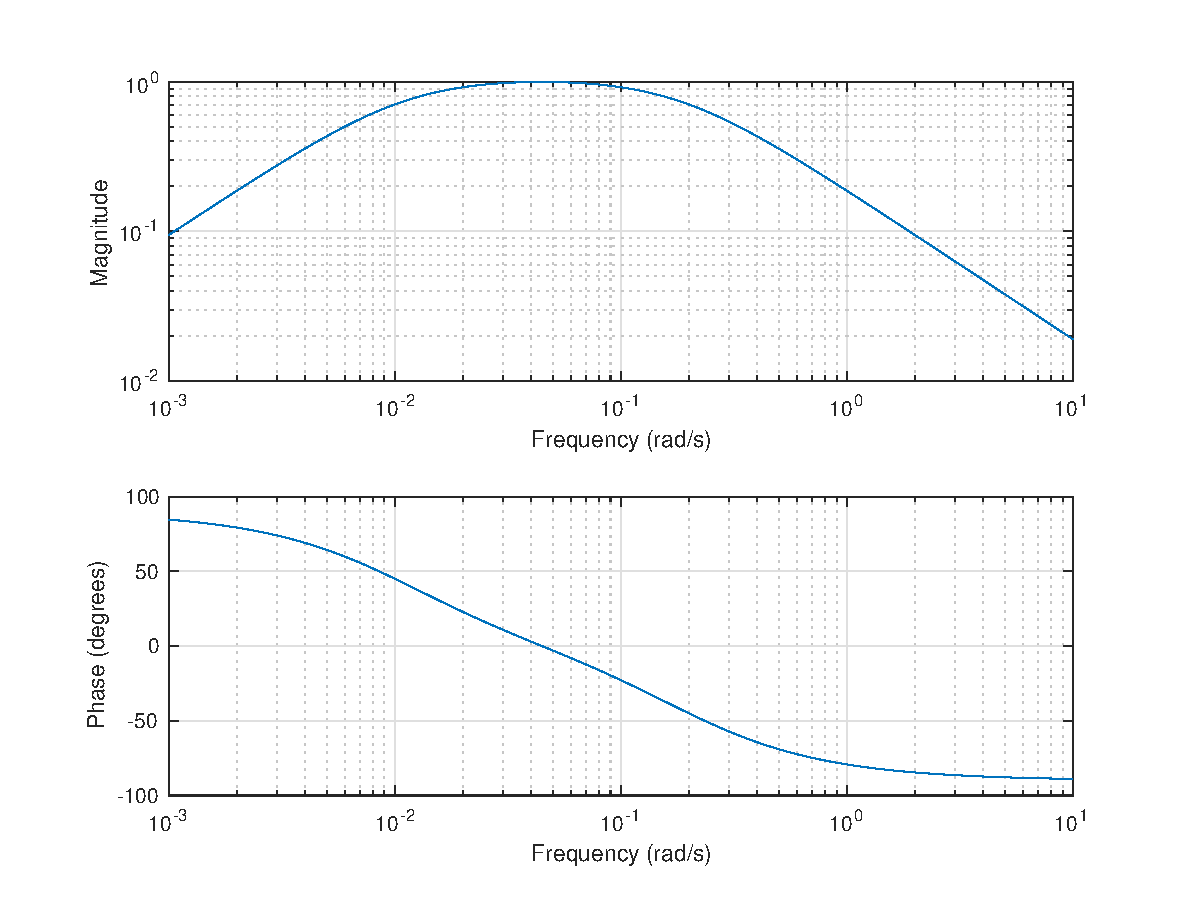
\includegraphics[width=\maxwidth{56.196688409433015em}]{figure_0.eps}
\end{center}


\begin{par}
\begin{flushleft}
In order to simulate real world conditions a circular zer mean noise is added to the originial system.
\end{flushleft}
\end{par}

\begin{par}
\begin{flushleft}
As one can see $G_0$ and $G_m$ share the same shape.
\end{flushleft}
\end{par}

\begin{matlabcode}
% Circular zero mean white noise
sigma = 0.001;          % Standard deviation
noise = sigma*(randn(N,1) + 1i*randn(N,1))/sqrt(2);

% Measured frequncy response
G_m = G_0 + noise;

figure;
plot(W,db(G_0));hold on;
plot(W,db(G_m));
legend('G_0(\omega_{k})','G_m(\omega_{k})');
title('Measured and real frequency response');grid on;
ylabel('Magnitude (dB)');xlabel('Frequency (rad/s)');
\end{matlabcode}
\begin{center}
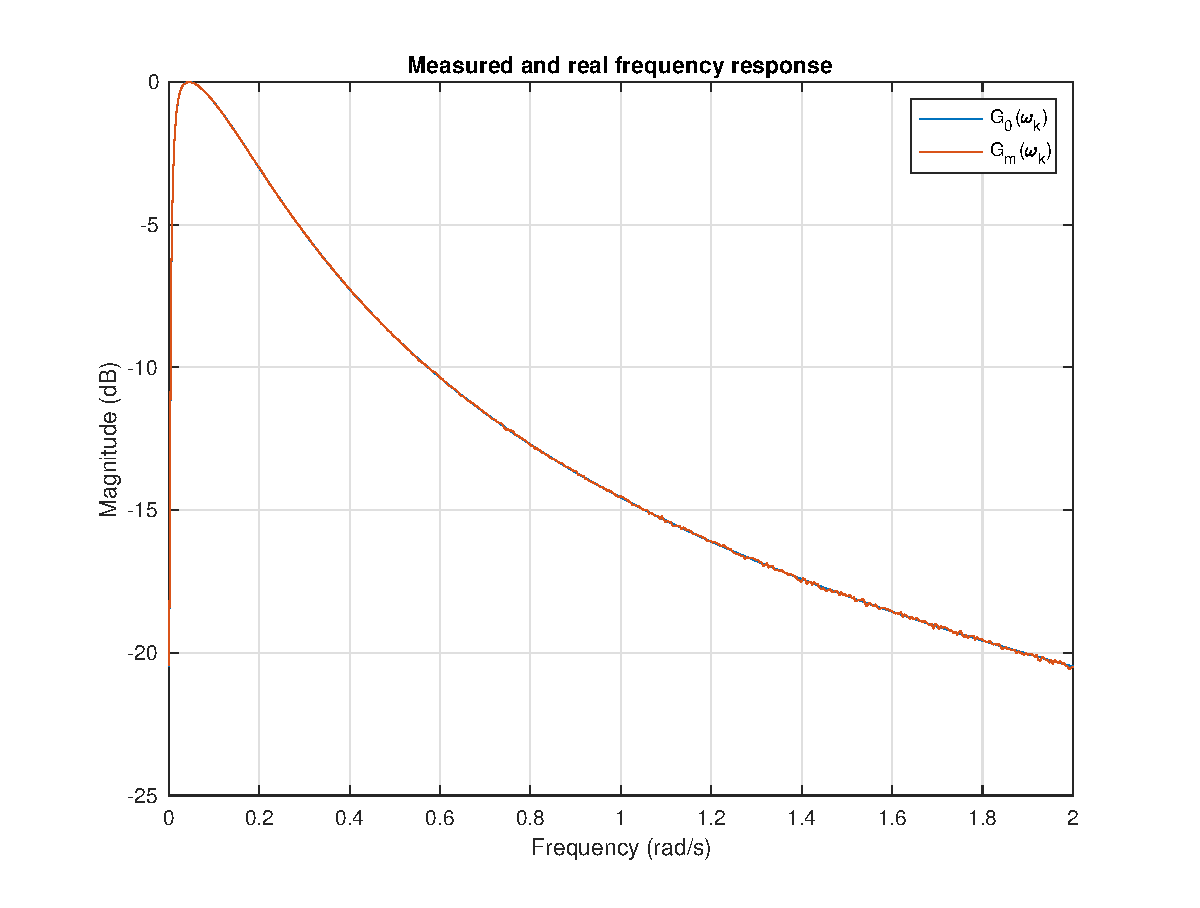
\includegraphics[width=\maxwidth{56.196688409433015em}]{figure_1.eps}
\end{center}


\begin{par}
\begin{flushleft}
Here the Laplacian s parameter is defined 
\end{flushleft}
\end{par}

\begin{matlabcode}
% Rewrite the transfer funciton
s = 1i*W;
s_all = s.^((0:length(B_tilde)-1));
s_all = fliplr(s_all);

\end{matlabcode}


\begin{par}
$$\begin{array}{l}
B(s,b)=b_2 s^2 +b_1 s+b_0 \\
A^{\prime } (s,a)=a_2 s^2 +a_1 s
\end{array}$$
\end{par}

\begin{matlabcode}
% Rewriten B and A' polynomials
B_true = polyval(B_tilde,s);
A_prime_true = polyval([A_tilde(1:2) 0],s);
\end{matlabcode}


\begin{par}
\begin{flushleft}
The real and measured frequency responses ares compared. The impact of the noise is clearly shown on the figure below.
\end{flushleft}
\end{par}

\begin{matlabcode}
% True parameters
theta_true = [B_tilde(1:3) A_tilde(1:2)];
theta_true = (theta_true).';

% Estimation figure
Bias = G_0 - G_m;
figure('Name','Impulse response comparaisons')
semilogx(W,db(G_0),W,db(G_m),'*',W,db(sigma*ones(N,1)),W,db(Bias))
legend('G_0','G_m','\sigma_{means}','Bias');
title('G_0 and G_m comparaison')
xlabel('Freq [rad]');
ylabel('Magn [dB]');
\end{matlabcode}
\begin{center}
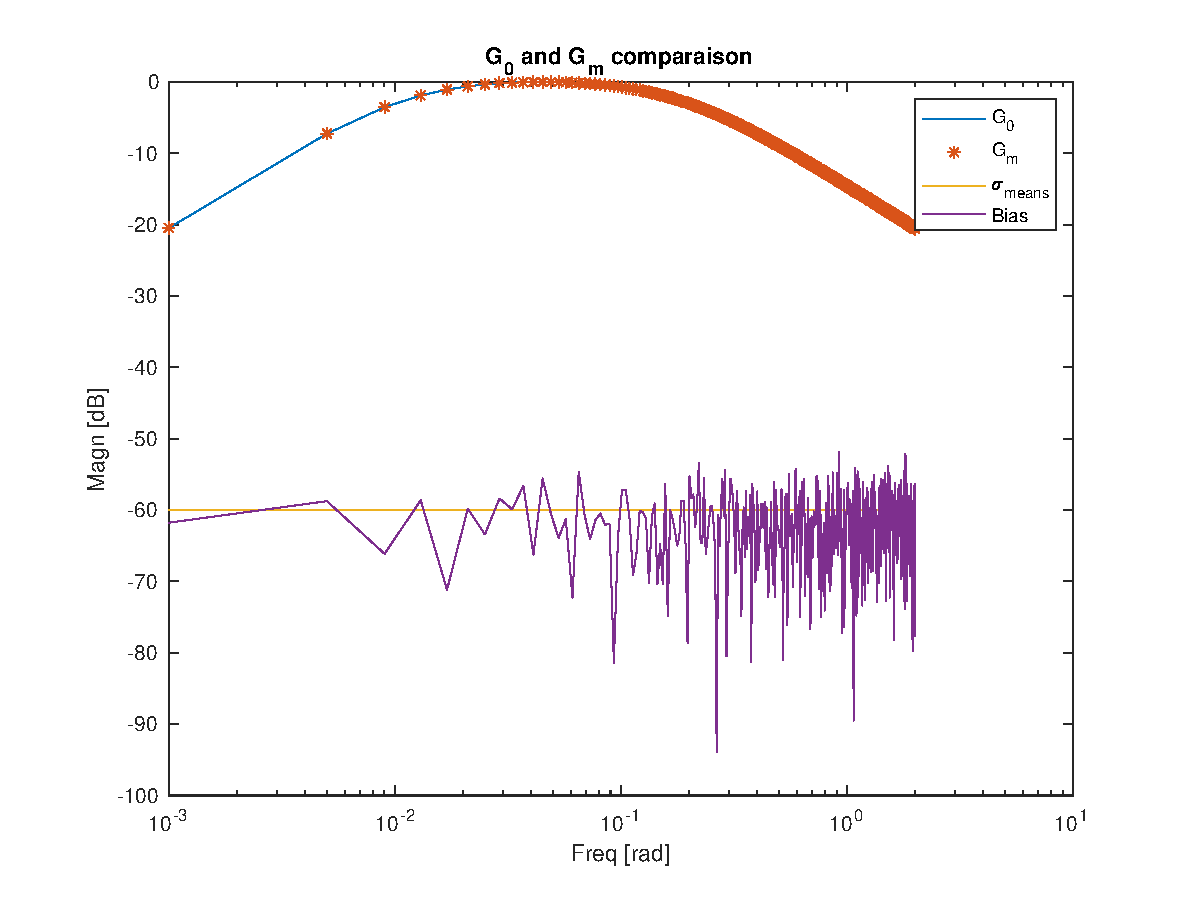
\includegraphics[width=\maxwidth{56.196688409433015em}]{figure_2.eps}
\end{center}


\begin{par}
\begin{flushleft}
\textbf{Implementation of the Levy estimators}
\end{flushleft}
\end{par}

\begin{par}
\begin{flushleft}
The Levy estimation should grow in precision while going up in the frequency domain. This coms from the fact that it correcponds to the least square estimation multiplied by the norm of the normalized A polynomial. The results below show clearly that in low frequencies the estimetion struggles to follow the real FRF but when going up in frequencies it becomes highly accurate. The estimation error falls down as  we go higher in frequencies. The results are the expected ones.
\end{flushleft}
\end{par}

\begin{matlabcode}
% Cost function vectorization
e_Levy = G_m ;

% Jacobian
J_Levy = [-s_all(:,1) -s_all(:,2) -s_all(:,3) G_m.*s_all(:,1) G_m.*s_all(:,2)];

% Real/imaginary part separation
e_Levy_IR = [real(e_Levy) ; imag(e_Levy)]; 
J_Levy_IR = [real(J_Levy) ; imag(J_Levy)];

% Levy theta estimation
theta_Levy = -J_Levy_IR\e_Levy_IR;

GestLevy = freqs(theta_Levy(1:3),[theta_Levy(4:5); 1],W);
% Mean sqare error
display(join(['Mean square error: ', num2str(immse(G_0,GestLevy))]));
\end{matlabcode}
\begin{matlaboutput}
Mean square error: 0.007465
\end{matlaboutput}
\begin{matlabcode}

figure;
plot(W,db(GestLevy),'o',W,db(G_m),'*',W,db(G_0),'+')
xlabel('Freq [rad]');
ylabel('Magn [dB]');
\end{matlabcode}
\begin{center}
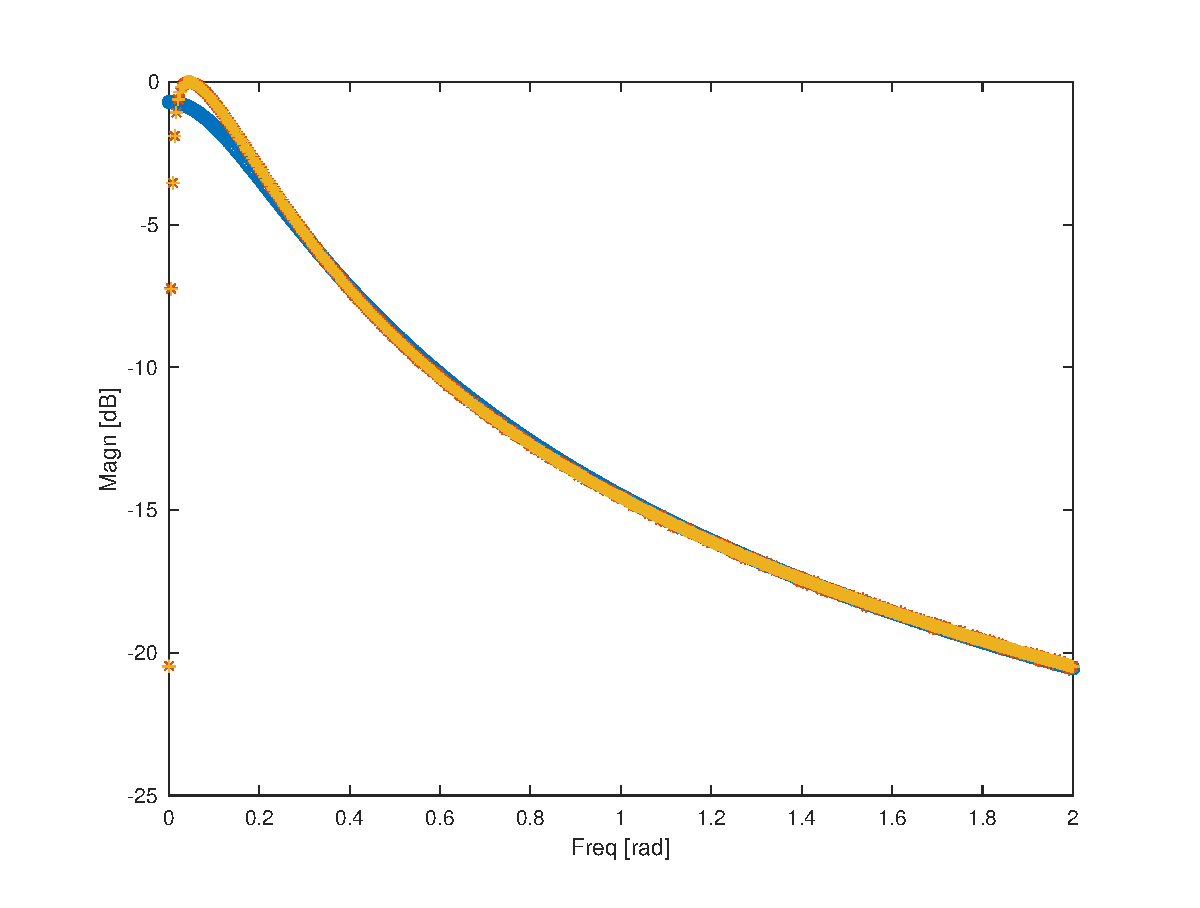
\includegraphics[width=\maxwidth{56.196688409433015em}]{figure_3.eps}
\end{center}
\begin{matlabcode}
% Estimation figure
deviation_0 = G_0 - GestLevy;
deviation_m = G_m - GestLevy;
figure('Name','Levy estimation')
% semilogx(W,db(GestLevy),W,db(G_m),'*',W,db(e_Levy),'+',W,db(sigma*ones(N,1)),W,db(deviation_0),W,db(deviation_m))
% legend('Levy estimation','G_m','e_{LS}','\sigma_{means}','e_{Levy0}','e_{Levy}')
semilogx(W,db(GestLevy),W,db(G_m),'*',W,db(std(G_m)*ones(N,1)),W,db(sigma*ones(N,1)),W,db(deviation_0),W,db(deviation_m),'+')
legend('Levy estimation','G_m','\sigma_{G_{m}}','\sigma_{means}','e_{Levy0}','e_{Levy}');
title('Levy estimation');
xlabel('Freq [rad]');
ylabel('Magn [dB]');
\end{matlabcode}
\begin{center}
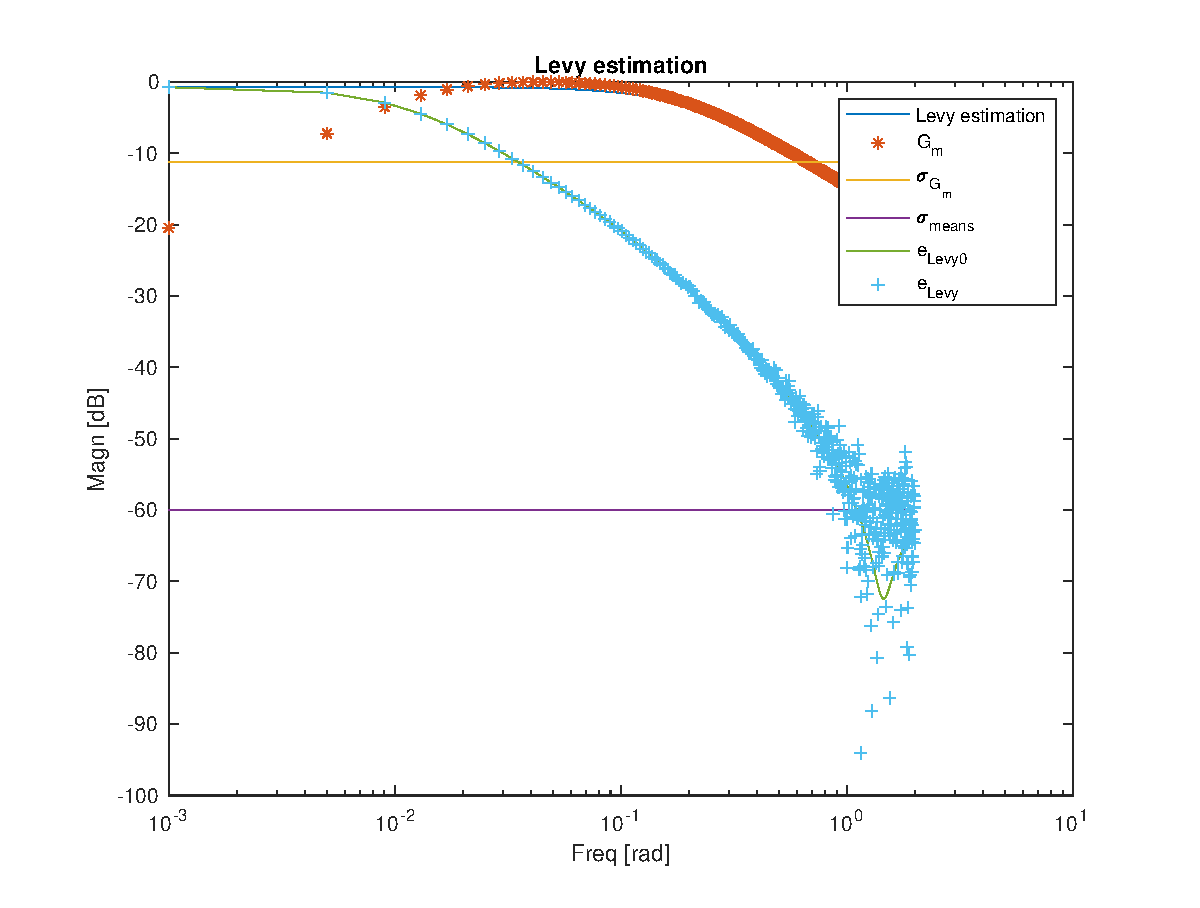
\includegraphics[width=\maxwidth{56.196688409433015em}]{figure_4.eps}
\end{center}
\begin{matlabcode}
disp('Parameters comparison'); 
\end{matlabcode}
\begin{matlaboutput}
Parameters comparison
\end{matlaboutput}
\begin{matlabcode}
disp(join(['True theta:           ',num2str(theta_true.')]));
\end{matlabcode}
\begin{matlaboutput}
True theta:           0   95    0  500   95
\end{matlaboutput}
\begin{matlabcode}
disp(join(['Levy estimated theta: ',num2str(theta_Levy(1:end).')]));
\end{matlabcode}
\begin{matlaboutput}
Levy estimated theta: 0.0090795      1.0756     0.92194      5.7131      5.8159
\end{matlaboutput}


\begin{par}
\begin{flushleft}
\textbf{Implementation of the Sanathanan estimator}
\end{flushleft}
\end{par}

\begin{par}
\begin{flushleft}
The results for the estimation using Sanathanan method are much more precise as it consist at minimizing a cost function which uses an approximation of the polynomial A at the denominator using an iterative algorithm. This way the Sanathanan cost functino resemble the original least square const function without sacrificing the linearity introduced by Levy. The better results are proven by the graphs and the mean square error measur which is considerably lower than the one in the Levy estimation. 
\end{flushleft}
\end{par}

\begin{par}
\begin{flushleft}
Again the approximation is more accurate in higher frequencies. However, even in lower frequencies the estimation error is lower than the standard deviation if the noise. This indicates that the estimation is closer to the original FRF than the one imapacted by the noise.
\end{flushleft}
\end{par}

\begin{matlabcode}
% Iteration index
l_San_max = 20;

% Computing B with new parameters
B = polyval(theta_Levy(1:3),s);

% Computing A with new parameters
A_prime = zeros(N,1);

% Cost function vectorization
e_San = G_m;

% Jacobian
J_San = J_Levy;

% Real/imaginary part separation
e_San_IR = [real(e_San) ; imag(e_San)]; 
J_San_IR = [real(J_San);imag(J_San)];

theta_San = zeros(5,1); 

% Sanathanan estimation
for l = 1:l_San_max
    
    % Parameters computation
    theta_San = -J_San_IR\e_San_IR;
    
    % Computing B with new parameters
    B = polyval(theta_San(1:3).',s);

    % Computing A with new parameters
    A_prime_new = polyval([theta_San(4:5).' 0],s);
    
    % Updating the cost function and the Jacobian
    e_San = G_m ./vecnorm(1+A_prime,2,2);
    J_San = J_Levy./vecnorm(1+A_prime,2,2);
    
    e_San_IR = [real(e_San) ; imag(e_San)]; 
    J_San_IR = [real(J_San) ; imag(J_San)];
    
    % Saving the previous A_prime
    A_prime = A_prime_new;
end

GestSan = freqs(theta_San(1:3),[theta_San(4:5); 1],W);
% Mean sqare error
display(join(['Mean square error: ', num2str(immse(G_0,GestSan))]));
\end{matlabcode}
\begin{matlaboutput}
Mean square error: 6.9475e-09
\end{matlaboutput}
\begin{matlabcode}

figure('Name','Sanathanan estimation')
plot(W,db(GestSan),'o',W,db(G_m),'*',W,db(G_0),'+')
legend('Sanathanan','G_m','G_0')
xlabel('Freq [rad]');
ylabel('Magn [dB]');
\end{matlabcode}
\begin{center}
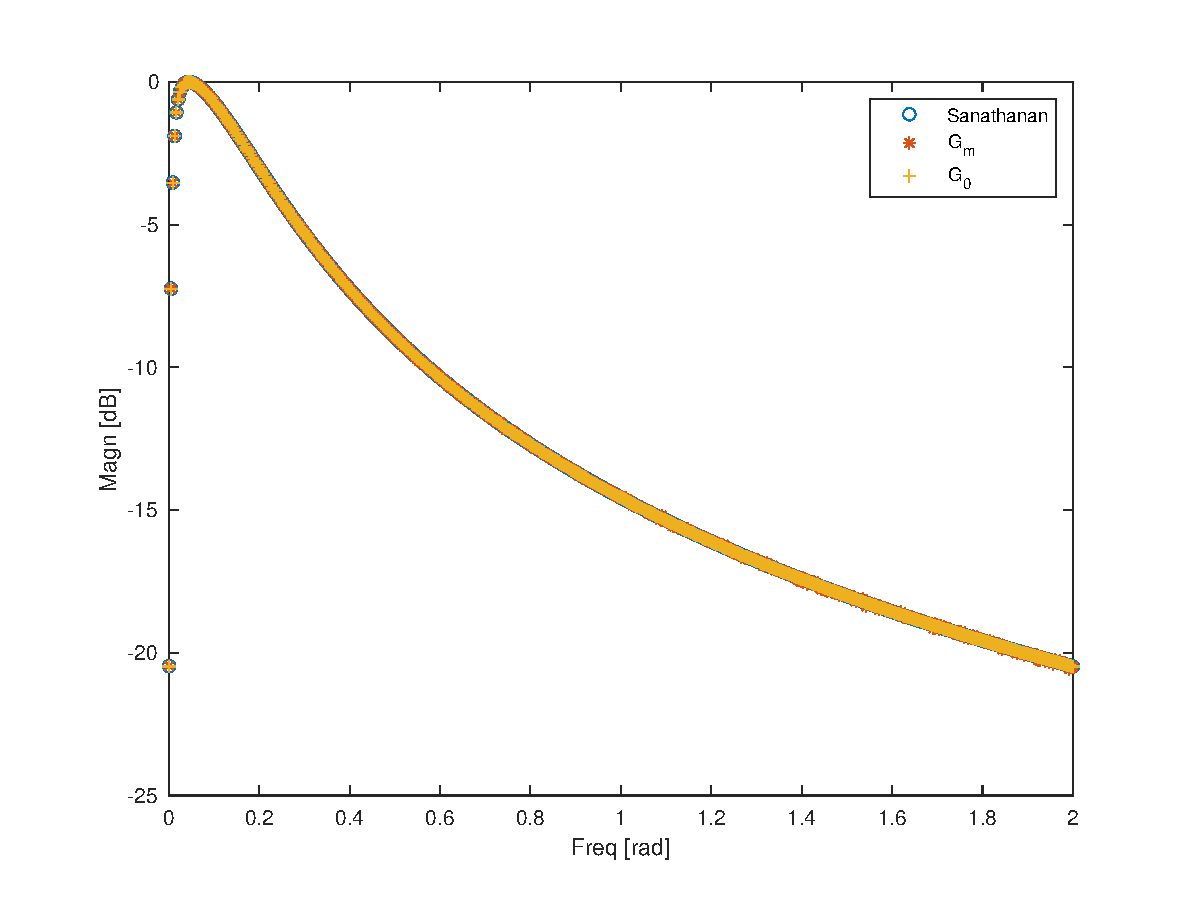
\includegraphics[width=\maxwidth{56.196688409433015em}]{figure_5.eps}
\end{center}
\begin{matlabcode}
% Estimation figure
stand_dev = std(G_m)
\end{matlabcode}
\begin{matlaboutput}
stand_dev = 0.2750
\end{matlaboutput}
\begin{matlabcode}
deviation_0 = G_0 - GestSan;
deviation_m = G_m - GestSan;
figure('Name','Sanathanan estimation')
semilogx(W,db(GestSan),W,db(G_m),'*',W,db(std(G_m)*ones(N,1)),W,db(sigma*ones(N,1)),W,db(deviation_0),'x',W,db(deviation_m),'+')
legend('Sanathanan estimation','G_m','\sigma_{G_{m}}','\sigma_{means}','e_{San0}','e_{San}')
title('Sanathanan estimation');
xlabel('Freq [rad]');
ylabel('Magn [dB]');
\end{matlabcode}
\begin{center}
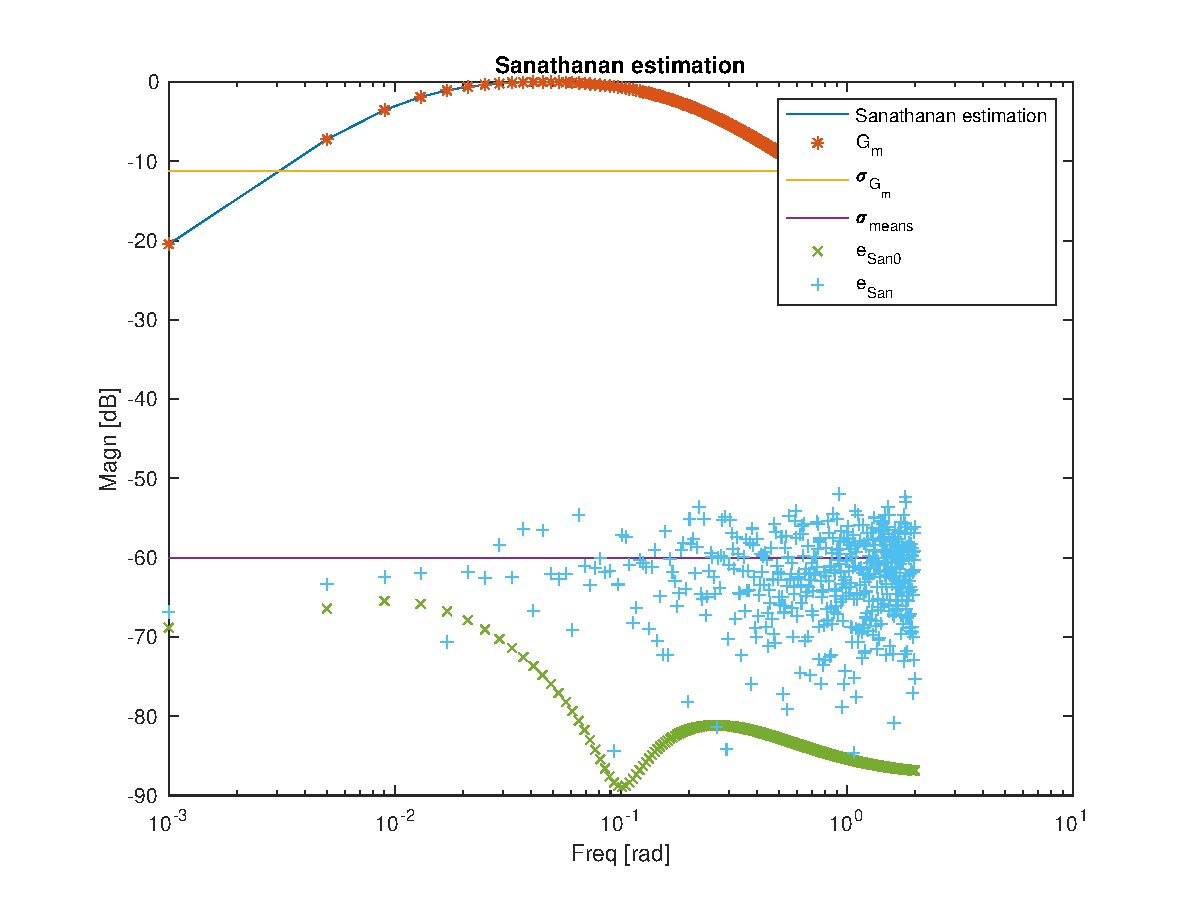
\includegraphics[width=\maxwidth{56.196688409433015em}]{figure_6.eps}
\end{center}
\begin{matlabcode}


disp(join(['Sanathanan estimated theta: ',num2str(theta_San.')]));
\end{matlabcode}
\begin{matlaboutput}
Sanathanan estimated theta: 0.02099346      95.12514 -0.0003531517      500.5868      95.12675
\end{matlaboutput}


\begin{par}
\begin{flushleft}
\textbf{Implemenating Gauss-Newton based least squares estimation}
\end{flushleft}
\end{par}

\begin{par}
\begin{flushleft}
Here a non linear estimator is implemented. Since it reduces the original cost function the results should be the best. The solution is obtained by using a iterative algorithm. 
\end{flushleft}
\end{par}

\begin{par}
\begin{flushleft}
The results are very close the the ones obtained with the Sanathanan estimator. In fact they seem indistinguishable ont the graphs. The only metric indicating a difference is the mean square error, but even there it is only $10^{-9}$.
\end{flushleft}
\end{par}

\begin{matlabcode}
% Initial parameters
theta_GN = theta_Levy;

% Number of iterations
l_GN_max = 20;

for l = 1:l_GN_max
    
    % Computing B with new parameters
    B = polyval(theta_GN(1:3).',s);

    % Computing A with new parameters
    A = polyval([theta_GN(4:5).' 1],s);
    
    % Cost function
    e_GN = G_m - B./A;
    
    % Jacobian
    J_GN = [-s_all(:,1) -s_all(:,2) -s_all(:,3) B.*s_all(:,1)./A B.*s_all(:,2)./A]./A;
    
    % Real values matrices
    e_GN_IR = [real(e_GN) ; imag(e_GN)]; 
    J_GN_IR = [real(J_GN) ; imag(J_GN)];
    
    % Delta theta
    delta_theta = -J_GN_IR\e_GN_IR;
    
    % Theta(l+1) = theta(l) + delta_theta
    theta_GN = theta_GN + delta_theta;
    
end

GestGN = freqs(theta_GN(1:3),[theta_GN(4:5); 1],W);
% Mean sqare error
display(join(['Mean square error: ', num2str(immse(G_0,GestGN))]));
\end{matlabcode}
\begin{matlaboutput}
Mean square error: 5.5913e-09
\end{matlaboutput}
\begin{matlabcode}

figure('Name','Maximum likelihood estimation')
plot(W,db(GestGN),'o',W,db(G_m),'*',W,db(G_0),'+')
legend('Maximum likelihood estimation','G_m','G_0')
xlabel('Freq [rad]');
ylabel('Magn [dB]');
\end{matlabcode}
\begin{center}
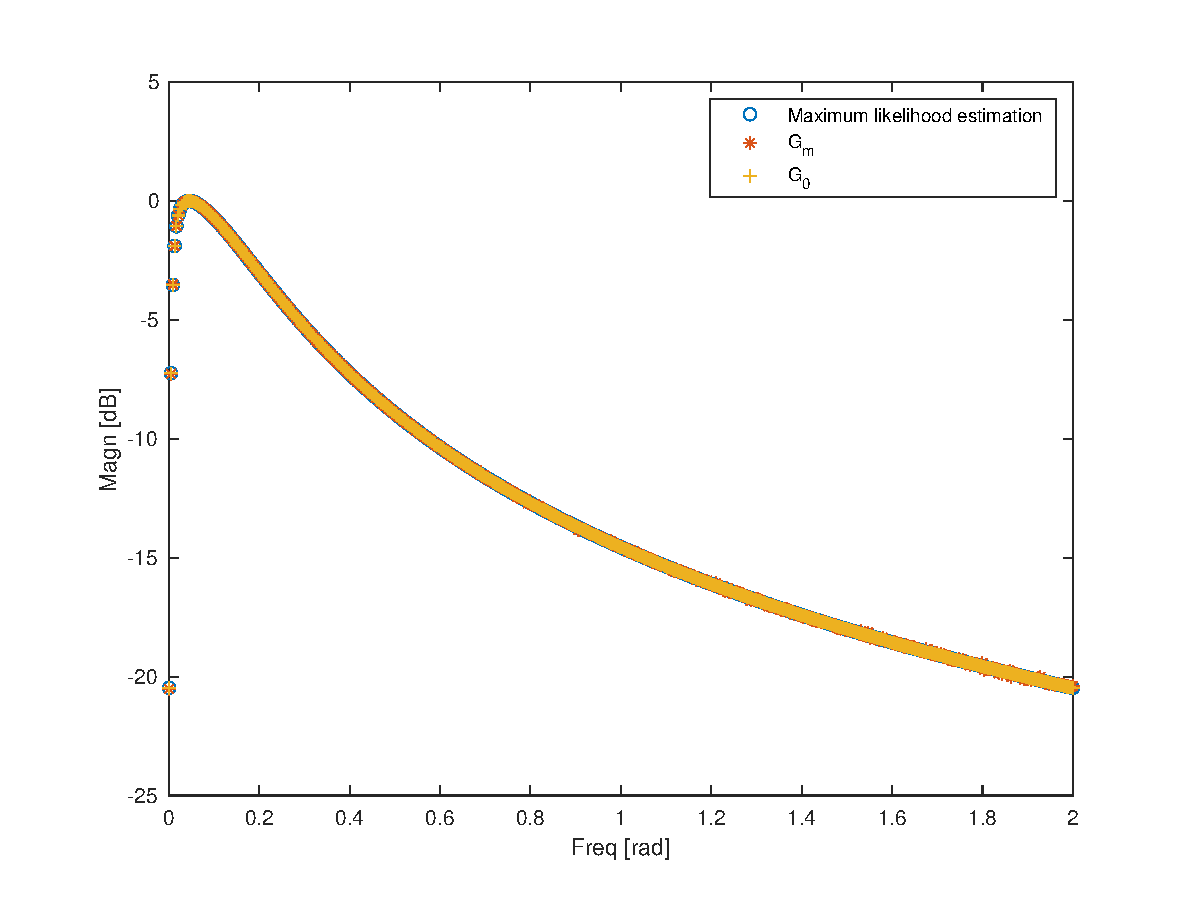
\includegraphics[width=\maxwidth{56.196688409433015em}]{figure_7.eps}
\end{center}
\begin{matlabcode}
% Estimation figure
deviation_0 = G_0 - GestGN;
deviation_m = G_m - GestGN;
figure('Name','Maximum likelihood estimation')
% semilogx(W,db(GestGN),W,db(G_m),'*',W,db(e_GN),'+',W,db(sigma*ones(N,1)),W,db(deviation_0),W,db(deviation_m))
% legend('Maximum likelihood','G_m','e_{LS}','\sigma_{means}','Bias')
semilogx(W,db(GestGN),W,db(G_m),'*',W,db(std(G_m)*ones(N,1)),W,db(sigma*ones(N,1)),W,db(deviation_0),W,db(deviation_m),'+')
legend('Maximum likelihood','G_m','\sigma_{G_{m}}','\sigma_{means}','e_{San0}','e_{San}')
title('Maximum likelihood estimation')
xlabel('Freq [rad]');
ylabel('Magn [dB]');
\end{matlabcode}
\begin{center}
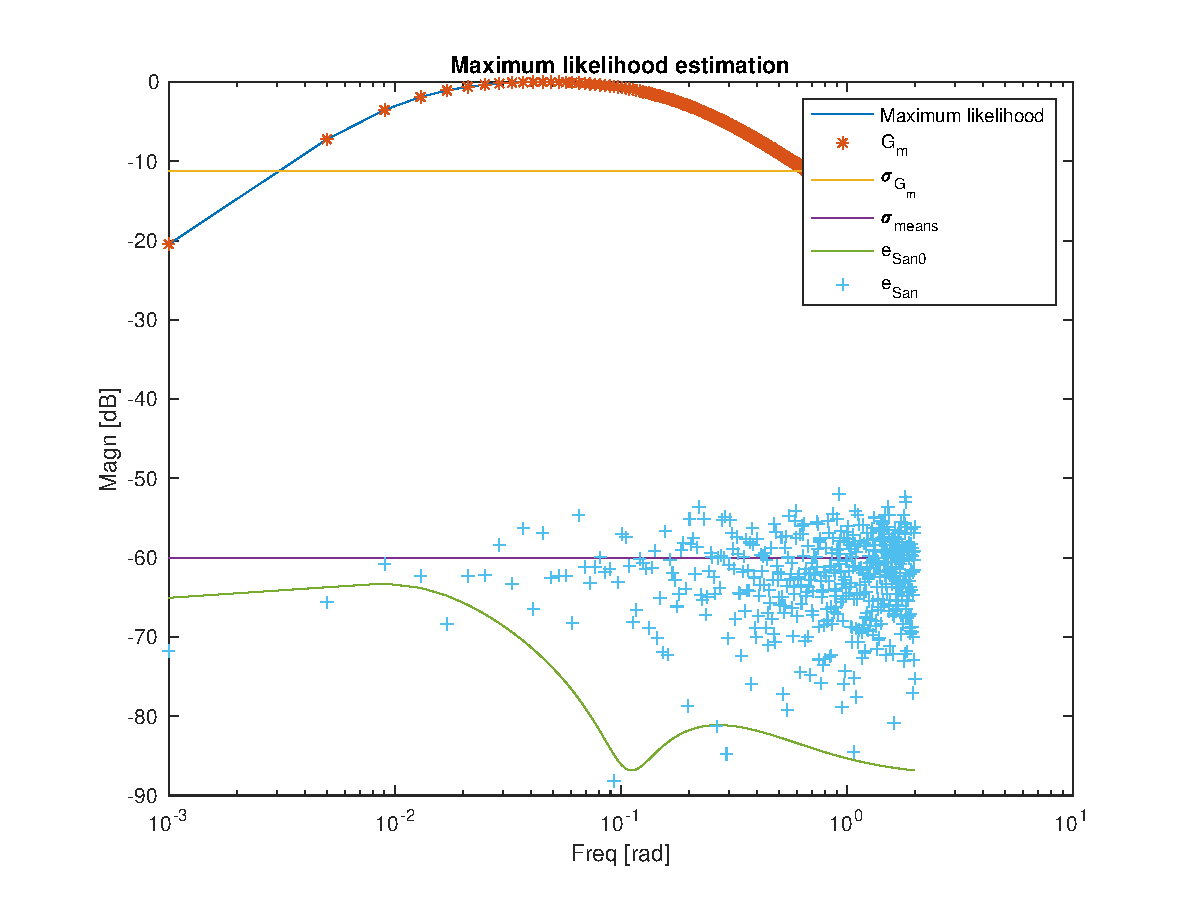
\includegraphics[width=\maxwidth{56.196688409433015em}]{figure_8.eps}
\end{center}

\end{document}
